\documentclass{article}


%%%%%%%%%%%%%%%%%%%%%%%%%%%%%%%%%%%%%%%%%%%%%%%%%%%%%%%%%%%%%%%%%%%%%%%%%%%%%%%%
%                                   Packages                                   %
%%%%%%%%%%%%%%%%%%%%%%%%%%%%%%%%%%%%%%%%%%%%%%%%%%%%%%%%%%%%%%%%%%%%%%%%%%%%%%%%

% LaTeX page and locale
\usepackage[utf8]{inputenc}
\usepackage[makeroom]{cancel}   
\usepackage{framed}             % Allows boxes around text
\usepackage{parskip}            % Prevents paragraphs from being indented
\usepackage{multirow}           % Allows cell merging row-wise in tables
\usepackage[margin=1.3in]{geometry} % Default margins make for tiny working 
                                % room for math. Make them smaller!

% Math-specific packages
\usepackage{amsmath}            % Allows fancy math stuff
\usepackage{amssymb}            % Fancy math letters

% Image and drawing specific packages
\usepackage{graphicx}           % Allows for images
\usepackage{tikz}               % Draws graphs

% Coding specific packages
\usepackage{minted}             % Allows pretty code blocks



%%%%%%%%%%%%%%%%%%%%%%%%%%%%%%%%%%%%%%%%%%%%%%%%%%%%%%%%%%%%%%%%%%%%%%%%%%%%%%%%
%                                    Macros                                    %
%%%%%%%%%%%%%%%%%%%%%%%%%%%%%%%%%%%%%%%%%%%%%%%%%%%%%%%%%%%%%%%%%%%%%%%%%%%%%%%%

% Front Page macros
\newcommand{\homeworktitle}{\uppercase{Homework 4}}
\newcommand{\homeworkauthor}{Charles Haithcock}
\newcommand{\unityid}{cehaith2}
\newcommand{\duedate}{Due: 21 April 2017}
\newcommand{\coursetitle}{CSC 505 - Design and Analysis of Algorithms}
\newcommand{\instructor}{Steffen Heber}

% Other macros
\newcommand\floor[1]{\lfloor#1\rfloor}  % floor function decorators
\newcommand\ceil[1]{\lceil#1\rceil}     % ceiling function decorators
\newcommand\separator{\rule{\textwidth}{.2pt}}  % separates solutions
\newcommand\encircle[1]{                % circles some text
  \tikz[baseline=(X.base)] 
    \node (X) [draw, shape=circle, inner sep=0] {\strut #1};}


%%%%%%%%%%%%%%%%%%%%%%%%%%%%%%%%%%%%%%%%%%%%%%%%%%%%%%%%%%%%%%%%%%%%%%%%%%%%%%%%
%                                   Title Page                                 %
%%%%%%%%%%%%%%%%%%%%%%%%%%%%%%%%%%%%%%%%%%%%%%%%%%%%%%%%%%%%%%%%%%%%%%%%%%%%%%%%

\begin{document}

\begin{center}
    \huge\textbf{\homeworktitle}
\end{center}
\vspace{1cm}

\begin{center}
    \large\homeworkauthor, \texttt{\unityid}
\end{center}
\vspace{1cm}

\begin{center}
    \large\coursetitle 
    
    \instructor
\end{center}
\vspace{1cm}

\begin{center}
    \large\duedate
\end{center}
\vspace{1cm}

\newpage



%%%%%%%%%%%%%%%%%%%%%%%%%%%%%%%%%%%%%%%%%%%%%%%%%%%%%%%%%%%%%%%%%%%%%%%%%%%%%%%%
%                                   Disclaimer                                 %
%%%%%%%%%%%%%%%%%%%%%%%%%%%%%%%%%%%%%%%%%%%%%%%%%%%%%%%%%%%%%%%%%%%%%%%%%%%%%%%%

Homework should be submitted using WolfWare Submit Admin in PDF, or plain text. 
To avoid reduced marks, please submit \textbf{word/latex-formated PDF file, NOT 
scanned writing in pdf format}. Scanned writing is hard to read, takes longer to
 grade, and produces gigantic files. \textbf{To simplify grading, please make 
sure that each problem starts on a new page}. All assignments are due on 9 PM of
the due date. Late submission will result in 10\%/40\% point reduction on the 
first/second day after the due date. No credit will be given to submission that 
are two or more days late. Please try out Submit Admin well before the due date 
to make sure that it works for you.

All assignments for this course are intended to be individual work. Turning in 
an assignment which is not your own work is cheating. The Internet is not an 
allowed resource! Copying of text, code or other content from the Internet (or 
other sources) is plagiarism. Any tool/resource must be approved in advance by 
the instructor and identified and acknowledged clearly in any work turned in, 
anything else is plagiarism.

General instruction about how to “give/describe/...” an algorithm, taken from 
Erik Demaine. \textbf{Try to be concise, correct, and complete.} To avoid 
deductions, you should provide (1) a textual description of the algorithm, and, 
if helpful, pseudocode; (2) at least one worked example or diagram to illustrate
how your algorithm works; (3) a proof (or other indication) of the correctness 
of the algorithm; and (4) an analysis of the time complexity (and, if relevant, 
the space complexity) of the algorithm. Remember that, above all else, your goal
is to communicate. If a grader cannot understand your solution, they cannot give
you appropriate credit for it.

\newpage

%%%%%%%%%%%%%%%%%%%%%%%%%%%%%%%%%%%%%%%%%%%%%%%%%%%%%%%%%%%%%%%%%%%%%%%%%%%%%%%%
%                                   Question 1                                 %
%%%%%%%%%%%%%%%%%%%%%%%%%%%%%%%%%%%%%%%%%%%%%%%%%%%%%%%%%%%%%%%%%%%%%%%%%%%%%%%%

\begin{framed}
    \textbf{Question 1 (24 pts, 3 pts each)}
    \begin{itemize}
        \item Problem 22-2 a-h (3 points each)
        
        \begin{quote}
            \textbf{\textit{22-2 Articulation points, bridges, and biconnected 
            components}}
            
            Let $G = (V, E)$ be a connected, undirected graph. An \textbf{
            \textit{articulation point}} of $G$ is a vertex whose removal 
            disconnects $G$. A \textbf{\textit{bridge}} of $G$ is an edge whose 
            removal disconnects $G$. A \textbf{\textit{biconnected component}} 
            of $G$ is a maximal set of edges such that any two edges in the set 
            lie on a common simple cycle. Figure 22.10 illustrates these 
            definitions. We can determine articulation points, bridges, and 
            biconnected components using depth-first search. Let $G_\pi = (V, 
            E_\pi)$ be a depth-first tree of $G$.
            
            \begin{enumerate}
                \item[\textbf{\textit{a.}}] Prove that the root of $G_\pi$ is an
                    articulation point of $G$ if and only if it has at least two
                    children in $G_\pi$
                \item[\textbf{\textit{b.}}] Let $v$ be a nonroot vertex of 
                    $G_\pi$. Prove that $v$ is an articulation point of $G$ if 
                    and only if $v$ has a child $s$ such that there is no back 
                    edge from $s$ or any descendant of $s$ to a proper ancestor 
                    of $v$. 
                \item[\textbf{\textit{c.}}] Let
                    \begin{align}
                        v.low = \text{min} 
                        \begin{cases}
                            v.d, \\
                            w.d: (u, w) \text{ is a back edge for some 
                                descendant } u \text{ of } v.
                        \end{cases}
                    \end{align}
                    Show how to compute $v.low$ for all vertices $v \in V$ in 
                    $O(E)$ time
                \item[\textbf{\textit{d.}}] Show how to compute all articulation
                    points in $O(E)$ time.
                \item[\textbf{\textit{e.}}] Prove that an edge of $G$ is a 
                    bridge if and only if it does not lie on any simple cycle of
                    $G$. 
                \item[\textbf{\textit{f.}}] Show how to compute all the bridges 
                    of $G$ in $O(E)$ time. 
                \item[\textbf{\textit{g.}}] Prove that the biconnected 
                    components of $G$ partition the nonbridge edges of $G$. 
                \item[\textbf{\textit{h.}}] Give an $O(E)$-time algorithm to 
                    label each edge $e$ of $G$ with a positive integer $e.bcc$ 
                    such that $e.bcc = e'$ if and only if $e$ and $e'$ are in 
                    the same biconnected component.
            \end{enumerate}
        \end{quote}
        \item Problem 22-3 a (4 points) on pages 622 and 623
        \begin{quote}
            \textbf{\textit{22-3 Euler tour}} 
            
            An \textbf{\textit{Euler tour}} of a strongly connected, directed 
            graph $G = (V, E)$ is a cycle that traverses each edge of $G$ 
            exactly once, although it may visit a vertex more than once. 
            \begin{enumerate}
                \item[\textbf{\textit{a.}}] Show that $G$ has an Euler tour if 
                    and only if in-degree($v$) = out-degree(v) for each vertex 
                    $v \in V$. 
            \end{enumerate}
        \end{quote}
    \end{itemize} 

    \separator
    
    \textit{Purpose} Learn about articulation points, bridges, biconnected 
    components, and Euler tours

\end{framed}

%%%%%%%%%%
% Answer %
%%%%%%%%%%


\textbf{Problem 22-2 a} 

The root, $r$, of a Depth-First Search (DFS) tree, $G_\pi$, can have thee 
different kinds of amounts of children; (a) zero children, (b) one child, (c) 
and two or more children. For (a), if $r$ has no children, $r$ is part of a 
graph of only one node, so removal of $r$ from $G_\pi$ will not disconnect the 
graph so $r$ is not an articulation point. For (b), if $r$ has only one child, 
then $r$ can reach all nodes and all nodes can reach each other without 
travelling through $r$. Removal of $r$ will never prevent any node from reaching
any other node (except of course $r$ itself) so $r$ is not an articulation 
point. 

For (c), assume $r$ has two children (the roots of subtrees $s_1$ and $s_2$) and
removal of $r$ would not disconnect the tree. In such a scenario where removal 
of $r$ does not disconnect $G_\pi$, a back edge must exist which connects the 
subtrees. Two problems exist with this however; by definition, trees do not 
contain cycles so $G_\pi$ would never have been a DFS tree to begin with. The 
second, more important aspect of such a contradiction is, when building $G_\pi$,
the required back edge would have been traversed first while exploring $s_1$ 
before going through $s_2$ and created a different DFS tree from $G_\pi$. This 
contradiction would extend for any number of subtrees $s_1, s_2, \ldots s_n$ as 
back edges would need to connects some node in $s_k$ to $s_{k-1}: 1 < k \le n$. 
As such, removal of $r$ would cause a disconnect graph meaning $r$ is an 
articulation point. QED. 

\separator

\textbf{Problem 22-2 b} 

Assume removal of $v$ would not disconnect $v$'s child $s$ or some descendant of
$s$, no back edge exists connecting $s$ or a descendant of $s$ to an ancestor of
$v$, and $v$ is a non-root vertex of $G_\pi$. In order for such a disconnect to 
be prevented, (1) an edge would need to exist connecting $s$ or the descendant 
of $s$ to some ancestor of $v$ or (2) to another node of $G_\pi$ not part of the
subtree whose root is $v$. The second scenario is impossible as such an edge 
would be traversed in an earlier visited subtree connected to via the cross 
edge. In order for (1) to operate, an edge would need to exist connecting $s$ or
some descendant of $s$ to some ancestor of $v$. Such an edge is by definition a
back edge, creating a contradiction. QED. 

\separator

\textbf{Problem 22-2 c} 

\textbf{Textual description of the algorithm with pseudocode}

Because the two main cases in the formula provided are either $v.d$, the current
vertex's discovery time, or consideration of backedges of descendants of $v$ if
they have back edges, the algorithm recurses down children before considering 
the $v.low$ by starting with leaves of subtrees and propagating the minimum 
values upward. 

On each recursion, the algorithm begins by assuming the minimum (\texttt{min}) 
is the current node, $v$'s discovery time, $v.d$ (case one in the formula). 
From here, backedges from $v$ are checked (if any) and compared to the current 
\texttt{min}, meaning the algorithm performs $\text{min}(v.d, w.d)$ where $w.d$
is the vertex on the other end of the back edge starting at $v$. All backedges
starting with $v$ are checked updating \texttt{min} along the way. The algorithm
assumes multiple backe dges can exist and assumes a function 
\texttt{back\_edges(v)} exists which takes a vertex \texttt{v} as a parameter 
and returns a list of backedges starting with \texttt{v} each with a pointer to
the node on the other end called \texttt{w}, similar to the formula. 

After checking all backedges starting from $v$, the children of $v$ are checked.
In order to accomplish the task of checking for the discovery time to 
descendants of $v$ to a backedge to $w$, the algorithm eventually returns
\texttt{min} for $v$ which allows for checking of descendants of $v$ which many
have backedges. The section above which checks for backedges and stores the
minimum of such (if applicable) allows propagating the value upward. If a
backedge does not exist, then a descendant $u$ of $v$ should have $u.d > v.d$ 
because the DFS algorithm discovers $u$ after $v$. For each child of $v$, the
\texttt{min} is appropriately updated if the returned $d$ time is lower than
\texttt{min}. 

Once all backedges and children of $v$ are checked, \texttt{min} is returned as
it should contain $v.d$. Returning $v.d$ allows for parent recursions to check
descendants. 

The algorithm is made recursive and given an ``entry point'' to facilitate 
recursion. 

\begin{minted}[
    framesep=2mm,
    baselinestretch=1.2,
    fontsize=\footnotesize,
    linenos
]{python}
def compute_low(G_pi):
    # Base case.
    _rec_compute_low(G_pi.V, G_pi.E, G_pi.root)

def _rec_compute_low(V, E, v):
    # Assume low is v.d until proven otherwise
    min = v.d

    # Gather min back_edge from children if applicable
    for u in children(v):  # does nothing if no children
        # Just grab first one or keep only the min back edge
        child_back_edge = _rec_compute_low(V, E, u)
        if child_back_edge.w.d < min:
            min = child_back_edge.w.d

    # Check if a back edge exists from us to some ancestor to propagate up
    # starting with the minimum child back edge propagated up to us
    for back_edge in back_edges(v):
        if back_edge.w.d < min: 
            min = back_edge.w.d

    # Update low if a back edge was found and is less than v.d
    v.low = min
    
    # return descendant.low or v.low up. NOTE if no back edge exists, 
    # v.low will be propagated up and v.low < parent v.low, so can safely
    # propagate up. 
    return min
\end{minted}


\textbf{A worked example}

Consider the following example DFS Tree where dotted edges are back edges and 
the vertices contain the vertex label and corresponding discovery/finish times. 

\begin{figure}[h]
    \centering
    \label{fig:my_label}
    \resizebox {.8\columnwidth} {!} {
    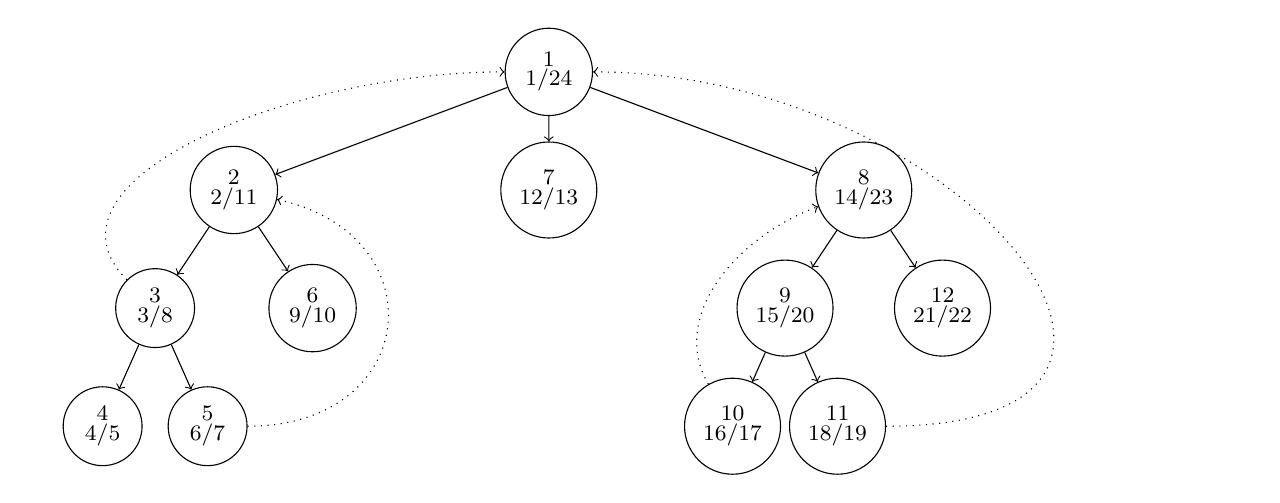
\begin{tikzpicture}[
            level/.style={->, sibling distance=4cm/#1, level distance = 1.5cm},
            n/.style={circle, draw, minimum size=.5cm, align=center},
            font={\fontsize{8pt}{5}\selectfont}
        ]
        \node[n] (1){1 \\ 1/24}  % node, what it looks like, name, contents
            child {node[n] (2) {2 \\ 2/11}
                child {node[n] (3) {3 \\ 3/8}
                    child {node[n] (4) {4 \\ 4/5}}
                    child {node[n] (5) {5 \\ 6/7}}
                }
                child {node[n] (6) {6 \\ 9/10}}
            }
            child {node[n] (7) {7 \\ 12/13}}
            child {node[n] (8) {8 \\ 14/23}
                child {node[n] (9) {9 \\ 15/20}
                    child {node[n] (10) {10 \\ 16/17}}
                    child {node[n] (11) {11 \\ 18/19}}
                }
                child {node[n] (12) {12 \\ 21/22}}
            }
        ;
        % Backedges
        %Form: 
        %  \draw[arrow, arrow style] (src) edge[out=pos on circle, in=pos on 
        %         circle] (dest);
        % pos on circle is degree of angle on circle with 0 being right most 
        %          point
        \draw[->, dotted] (3) edge[out=120, in=180, xscale=2] (1);
        \draw[->, dotted] (5) edge[out=0, in=340, xscale=2] (2);
        \draw[->, dotted] (10) edge[out=120, in=200] (8);
        \draw[->, dotted] (11) edge[out=0, in=0, xscale=2, yscale=.8] (1);
    \end{tikzpicture}
    }
\end{figure}

Below are the recursions in the algorithm: 

\begin{center}
\begin{tabular}{ |c|c|l|c|c| } 
    \hline
    $v$ & 
        $v.d$ & 
        Recurse & 
        \texttt{back\_edges(v)} & 
        $v.low$ \\ 
    \hline
    
    1 & 
        1 & 
        \{\encircle{2}: \cancel{1}, \encircle{7}: $\O$, \encircle{8}: 
            \cancel{1}\} & 
        $\O$ & 
        1 \\
    \hline
    
    2 & 
        \cancel{2} & 
        \{\encircle{3}: 1, \encircle{6}: \cancel{9}\} & 
        $\O$ &
        1 \\
    \hline
    
    3 & 
        \cancel{3} &
        \{\encircle{4}: \cancel{4}, \encircle{5}: \cancel{2}\} & 
        \{(3, 1).w.d = 1\} &
        1 \\
    \hline
    
    4 & 
        4 & 
        $\O$ & 
        $\O$ &
        4 \\
    \hline
    
    5 & 
        \cancel{6} &
        $\O$ & 
        \{(5, 2).w.d = 2\} &
        2 \\
    \hline
    
    6 & 
         9 & 
         $\O$ & 
         $\O$ &
         9 \\
    \hline
    
    7 & 
        12 &
        $\O$ & 
        $\O$ & 
        12 \\
    \hline
    
    8 & 
        \cancel{14} &
        \{\encircle{9}: 1, \encircle{12}: \cancel{21}\} &
        $\O$ &
        1 \\
    \hline
    
    9 & 
        \cancel{15} &
        \{\encircle{10}: \cancel{14}, \encircle{11}, 1\} & 
        $\O$ & 
        1 \\
    \hline
    
    10 & 
        \cancel{16} & 
        $\O$ & 
        \{(10, 8).w.d = 14\} &
        14 \\
    \hline
    
    11 & 
        \cancel{18} &
        $\O$ & 
        \{(11, 1).w.e = 1\} &
        1 \\
    \hline
    
    12 & 
        21 &
        $\O$ & 
        $\O$ &
        21 \\
    \hline
\end{tabular}
\end{center}

Note the table is layed out as if after having ran the entirety of the 
algorithm. As values are checked, if it does not cause an update to \texttt{min}
or if the prior \texttt{min} is replaced, its value will be crossed out. 

\textbf{Proof}

For the loop at lines 10-14, the loop begins with no children being explored. At
some later iteration before termination, at least one child of $v$ has been 
recursed on where in each child in the interim should have passed up its 
respective \texttt{min} value. $v$'s \texttt{min} currently should be the 
lowest value when comparing $v.d$ and $v$'s children $low$ for ones explored so
far. Line 13 ensures the lowest $low$ value is kept. Upon termination,
\texttt{min} will be the lowest value among \{$v.d, c_0, c_1, \ldots, c_n$\} 
where $c_0$ through $c_n$ are children of $v$. If some $c_i.low > v.low$, then 
$c_i$ does not have have a back edge from itself or a descendant to an ancestor
of itself. 

The loop at lines 18-20 check for any back edges from $v$ to an ancestor of $v$.
Only $v$ needs to be checked, because, by walking through the children of $v$ 
and keeping the smallest $low$ value respectively, if $v$ has a descendant, $u$,
with a back edge to an ancestor of $v$, then $u.low \le v.d < u.d$. Upon 
starting the loop, \texttt{min} will still be lowest value among \{$v.d, c_0, 
c_1, \ldots, c_n$\}. During the $i^{th}$ iteration, if a back edge exists which
points to an ancestor of $v$ with an earlier discovery time then a prior back
edge whose discovery time was propagated up via the first loop, then 
\texttt{min} will be updated with the appropriate discovery time among the
$i-1$ back edges which have already been investigated. Upon termination, all 
back edges from $v$ are searched and line 19 ensures the back edge to the 
earliest vertex is kept. 

\textbf{Time complexity analysis}

Assuming all operations are constant time actions, the loops at lines 10-14 and
18-20 are thus multiple iterations of constant time actions. Likewise, these 
loops are ran for each recursion. A recursion occurs for each node in the graph.
As such, for the recursions alone, the algorithm is guaranteed to run at 
$\Theta(|V|)$. 

In general, for every node, all possible edges are eventually considered; when 
checking all children of a node, all edges connected via tree edges are 
considered followed up with a check against all back edges. As such, since the 
$|E|$ is typically greater than $|V|$, checking all edges dominates the running 
time over $|V|$. Thus the running time is bound at $O(|E|)$. 

\separator

\textbf{Problem 22-2 d} 

Fortunately, computing all articulation points is all but done with the above 
problems. The steps then are effectively layed out already;

\begin{enumerate}
    \item Run DFS against the graph, $G$, to generate $G_\pi$. This action 
        requires $O(|V|+|E|)$, however, since $G$ is connected, $|E| > |V| - 1$,
        so generating $G_\pi$ is only $O(|E|)$. 
    \item Run the above algorithm to calculate \texttt{low} for each vertex $v 
        \in V$.
    \item From here, with $G_\pi$, we can apply some of the above points to 
        determine articulation points in $G$. For each vertex $v \in V$:
    \begin{itemize}
        \item if $v$ is a root vertex and has more than one child, then $v$ is 
            an articulation point.
        \item if $v$ a non-root vertex, has descendants, and has no backedge to 
            a proper ancestor, $v$ is an articulation point. 
        \item if $v.d < $ any child of $v$, $u$'s $low$ value, then a back edge 
            must exist from $u$ to some proper ancestor of $v$. As such, if 
            $u.low \le v.d$, then a backedge does not exist meaning $v$ is an 
            articulation point. 
    \end{itemize}
\end{enumerate}

Because of the above, articulation points can be determined as the algorithm is 
performed. For example, each vertex can include an addition member in their 
structs named "is\_art\_point", a boolean value where true means the vertex is 
an articulation point (and false otherwise). On each iteration, simply check 
the current vertex, $v$, to see if $v$ has no parent pointer and has multiple 
children (case 1 above); if $v$ has a parent pointer, has children, and does not
contain a back pointer (case 2); and, on checking children, simply store the 
maximum $low$ value in all children and compare the $v.d$ with this maximum low 
value (case 3). If any of the cases are true, then $v$ is an articulation point 
and \texttt{v.is\_art\_point = True}. 

This modification adds no additional loops or recursions or any particulat 
actions which can not be represented in a single operation. As such, calculating
all articulation points does not change the running time of the algorithm. 

\separator

\textbf{Problem 22-2 e} 

Assume some edge, $e \in V$ is a bridge edge but is also part of a cycle of G. 
This implicates some vertex $v_i$ is able to reach some other vertex $v_j$ via 
$e$. If $e$ is indeed a bridge edge, then removal of $e$ from the graph will cut
the path between $v_i$ and $v_j$. However, despite the original path being 
destroyed by the removal of $e$, because $e$ lies in a cycle, an alternate path 
exists for $v_i$ to reach $v_j$. 

Inherently, if a path lies does not lie in a cycle, then some set of vertices 
have a path that must include said path to reach a separate set of vertices in 
the graph. Removal of the edge would destroy this path and any path which 
constitute the edge. However, if an edge lies on a cycle then every vertex can 
reach every other vertex in the cycle via the edges which constitute the cycle. 
If an edge is removed, every vertex can still reach every other vertex. As such,
any additional vertices or subtrees attached to the cycle before the edge 
removal will still be able to reach each other via different paths if an edge is
removed from the cycle. 

\separator

\textbf{Problem 22-2 f} 

Fortunately, $G_\pi$ can be used rather than $G$ for determining all bridges of 
$G$; a bridge, when removed, disconnects a graph. In a DFS, if a tree edge is 
removed, the vertices on either end, $u, v$ can not longer reach each other,
disconnecting the graph. So all bridges within $G$ will also exist within 
$G_\pi$. 

With the algorithm to calculate \texttt{low} for all vertices, the vertices, 
$v.d$ and $v.low$ can be used to determine bridges. In general, a series of 
edges with the same \texttt{low} score will end up being part of a simple cycle
of $G$ due to the \texttt{low} value being propagated up from a descendant with 
a back edge. When traversing $G_\pi$ looking for cycles, series of ancestrally 
related vertices with the same \texttt{low} value are part of a cycle until a 
parent vertex which has a different \texttt{low} value. The last child vertex 
in question then is also the end point of the back edge which caused all 
intermediate vertices to have the same \texttt{low} value. As such, the vertex,
$v$, should have $v.d = v.low$. 

The condition, $v.d = v.low$ can be used to determine bridges. The edge 
connecting $v$ with its predecessor then is an edge which connects a vertex in 
a simple cycle or as a leaf vertex to another vertex. This can be determined 
just at the end of a recursion where $v.low$ is assigned. If $v.d = v.low$, then
the edge connecting $v$ to its predecessor (if $v$ is not the root of $G_\pi$)
is a bridge edge. This adds no extra complexity to the algorithm beyond a check
for equivalencies for two prior known values and an assignment statement of a
single value to a single variable. 

\separator

\textbf{Problem 22-2 g} 

Similar to prior questions, the proof is built from conclusions drawn from 
answers \textbf{\textit{a.}} through \textbf{\textit{f.}}. From (e), any bridge
edge is already proven to not be a part of some simple cycle. Therefore, any 
non-bridge edge must be part of a simple cycle. By definition non-bridge edges,
since they must be a part of a simple cycle, must also always be a part of a 
biconnected component. 

To partition non-bridge edges means non-bridges can belong to only one 
biconnected component at a time. To prove biconnected components partition 
non-bridge edges via contradiction, assume some edge $e$ resides within multiple
biconnected components, $B_1$ and $B_2$. 

In order for disparate biconnected components to exist in a connected graph, 
$G$, the biconnected components must be connected via bridge edges otherwise the
biconnected components would be connected via edges which lie on cycles and 
cause the disparate biconnected components to collapse into each other causing
two biconnected components to become one biconnected component. 

That being said, if $e$ is to belong to $B_1$ and $B_2$, either end of $e$ could
be removed and $B_1$ and $B_2$ would not become disconnected (increasing the 
amount of connected components, contradicting the definition of a bridge edge. 
Furthermore, $B_1$ and $B_2$ would collapse into each other if $e$ were part of
both. As such, any non-bridge edge $e$ can be a part of only one biconnected 
component at a time. 

\separator

\textbf{Problem 22-2 h} 

The solution builds from the prior work and is quite simple. The algorithm 
described in (a) can be extended. Simply copy $G_\pi$ into a variable to mark 
each $e.bcc$, called $G_{bcc}$ and, when detecting bridges, simply remove the 
bridge from $G_{bcc}$. Once all bridges are removed, simply re-run DFS against
$G_{bcc}$ which will produce a forest of DFS trees. Here, traverse each tree and 
mark the corresponding edges in $G$ appropriately, wherein $e.bcc$ could simply
be the index of the tree. 

This works because, when removing all bridges, all biconnected components will 
remain, but the graph will become disconnected due to the property that bridges
can not lie on a cycle and are therefore not part of biconnected components and
removal of bridges will disconnect the graph. 

The algorithm in (a) runs in $O(|E|)$, so re-running DFS against $G_{bcc}$ will
incur an additional $O(|V|)$. Because $G_{bcc}$ is now disconnected before 
running DFS against it, $|V| > |E|$ rather than in previous iterations where DFS
runs at $O(|E|)$. 

\textbf{Problem 22-3 a} 

Assume $G$ indeed already has a cycle involving vertices $\{v_j, v_{j+1}, 
\ldots, v_k\}$. Such a cycle implies each vertex in this cycle has an edge to 
its sibling. For a directed graph, in order for a cycle to exist, each node must
be reachable to every other node in the cycle via some path made of some or all
the edges that constitutes the cycle. For here, the edges leading from a source 
vertex are "out-edges" while edges leading to a node are "in-edges". "In-degree"
then is the count of incoming edges whie "out-degree" is the count of outgoing 
edges. 

In the most simple example of a cycle within a directed graph, $G = \{v_1 , 
v_2\}$ such that $e_1 = edge(v_1 , v_2), e_2 = edge(v_2, v_1) $. The cycle 
created herein is then an Euler Tour because all edges in $G$ are able to be 
visited exactly once. For each vertex in $G$, the in-degree is 1 while 
out-degree is also 1 thus fitting the restriction of Euler's Tour where the 
in-degree for some vertex $v$ must equal the out-degree for that same vertex $v$
for all vertices in $G$. 

This example can be extended with arbitrarily large amounts of paths and 
vertices. In continuing the example, let $e_3 = edge(v_1, v_2): e_3 \cancel{=} 
e_1$. Here, while the Euler Tour still exists between $v_1$ and $v_2$ via $e_1$ 
and $e_2$, $e_3$ can not be a part of the same Euler Tour; to maintain a cycle, 
the path must traverse through the previously visited edge $e_2$ and doing so 
violates a condition of Euler Tours. However, if $e_4 = edge(v_2, v_1), e_4 
\cancel{=} e_2$, then the properties of Euler Tours are not violated. In the 
violation scenario, $in\_degree(v_1) = 1, out\_degree(v_1) = 2$ and vice-versa 
for $v_2$. Adding the forth path remedied the situation causing $in\_degree(v_1)
= out\_degree(v_1)$. 

Inherently, for any node, $v \in V$, for a directed graph $G$, if $G$ is a Euler
 Tour, $in\_degree(v) = out\_degree(v)$ otherwise a path exists to leave a node 
 and never return to the node. Consider the violation example above, the 
 out-degree did not match the in-degree for $v_1$ so, while the cycle persisted 
 due to $e_1$ and $e_2$, taking $e_3$ means taking a path that would prevent 
 returning to $v_1$ via edges which have yet to be traversed. 

In general, when $in\_degree(v) < out\_degree(v)$, a possible path exists where 
you can never return to $v$ if all edges are traversed in $G$. 

The other scenario is $in\_degree > out\_degree(v)$. In such a scenario, if all 
edges are to be traversed, eventually, $v$ would be reached via one of the 
in-edge but all of its out-edges would be exhausted. So the path terminates with
$v$. 



\newpage




%%%%%%%%%%%%%%%%%%%%%%%%%%%%%%%%%%%%%%%%%%%%%%%%%%%%%%%%%%%%%%%%%%%%%%%%%%%%%%%%
%                                   Question 2                                 %
%%%%%%%%%%%%%%%%%%%%%%%%%%%%%%%%%%%%%%%%%%%%%%%%%%%%%%%%%%%%%%%%%%%%%%%%%%%%%%%%

\begin{framed}
    \textbf{Question 2 (8 pts total)}
    
    Please sole problem 23-4 on page 641. You do NOT have to describe the most 
    efficient implementation of each algorithm.
    
    \begin{quote}
        \textbf{\textit{23-4 Alternative minimum-spanning-tree algorithms}} 
        
        In this problem, we give pseudocode for three different algorithms. Each
        one takes a connected graph and a weight function as input and returns a
        set of edges $T$. For each algorithm, either prove that $T$ is a minimum
        spanning tree or prove that $T$ is not necessarily a minimum spanning 
        tree. Also describe the most efficient implementation, whether or not it
        computes a minimum spanning tree. 
        
        \begin{enumerate}
            \item[\textbf{\textit{a.}}] MAYBE-MST-A$(G, w)$
\begin{minted}[  % For some reason, minted will pick up all tabs and spaces
    framesep=2mm,
    baselinestretch=1.2,
    fontsize=\footnotesize,
    linenos
]{c}
sort the edges into nonincreasing order of edge weights w
T = E
for each edge e, taken in nonincreasing order by weight:
    if T - {e} is a connected graph:
        T = T - {e}
return T
\end{minted}
            \item[\textbf{\textit{b.}}] MAYBE-MST-B$(G, w)$
\begin{minted}[  % For some reason, minted will pick up all tabs and spaces
    framesep=2mm,
    baselinestretch=1.2,
    fontsize=\footnotesize,
    linenos
]{c}
T = []
for each edge e, taken in arbitrary order:
    if T with {e} has no cycles:
        T = T with {e}
return T
\end{minted}            
            \item[\textbf{\textit{c.}}] MAYBE-MST-C$(G, w)$
\begin{minted}[  % For some reason, minted will pick up all tabs and spaces
    framesep=2mm,
    baselinestretch=1.2,
    fontsize=\footnotesize,
    linenos
]{c}
T = []
for each edge e, taken in arbitrary order:
    T = T with {e}
    if T has a cycle c:
        let e' be a maximum-weight edge on c:
        T = T - {e'}
return T
\end{minted}
        \end{enumerate}
    \end{quote}

    \separator

    \textit{Purpose} Reinforce your understanding of minimum spanning trees
\end{framed}


%%%%%%%%%%
% Answer %
%%%%%%%%%%

\textbf{MAYBE-MST-A}

MAYBE-MST-A is an implementation of Kruskal's algorithm but in reverse; 
Kruskal's algorithm begins with no edges and gradually adds then in order of 
increasing weight until all edges are checked while MAYBE-MST-A starts with all
edges possible and removes one at a time in order of decreasing weight until all
edges are checked. Neither would leave cycles. 

\separator

MAYBE-MST-B is similar in implementation to Kruskal's algorithm except it 
MAYBE-MST-B lacks any intelligent weight checking. The issue herein essentially
is the possibility only the heaviest of edges are added to $T$ even if $T$ is
still a spanning tree. In fact, the check in line 3 will actually allow $T$ to 
become a spanning tree. Again, however, since MAYBE-MST-B lacks consideration 
for weights, $T$ could be a Minimal Spanning Tree, but, in other iterations of
the algorithm, could produce a Maximal Spanning Tree and spanning trees of 
arbitrary weights. 

\separator



\newpage




%%%%%%%%%%%%%%%%%%%%%%%%%%%%%%%%%%%%%%%%%%%%%%%%%%%%%%%%%%%%%%%%%%%%%%%%%%%%%%%%
%                                   Question 3                                 %
%%%%%%%%%%%%%%%%%%%%%%%%%%%%%%%%%%%%%%%%%%%%%%%%%%%%%%%%%%%%%%%%%%%%%%%%%%%%%%%%

\begin{framed}
    \textbf{Question 3 (6 pts)}

    Suppose you have a weighted, undirected graph $G$ with positive edge weights
    and a start vertex $s$. Describe a modification of Dijkstra’s algorithm that 
    runs (asymptotically) as fast as the original algorithm, and assigns a label 
    $usp[u]$ to every vertex $u$ in $G$, so that $usp[u]$ is true if and only if 
    there is a unique shortest path from $s$ to $u$. By definition $usp[s]$ is 
    true. In addition to your modification, be sure to provide arguments for 
    both the correctness and time bound of your algorithm, and an example.
    
    \separator

    \textit{Purpose} Reinforce your understanding of Dijkstra’s shortest path 
    algorithm, and practice algorithm design
    
\end{framed}


%%%%%%%%%%
% Answer %
%%%%%%%%%%

\textbf{Textual description of the algorithm with pseudocode}

\begin{minted}[
    framesep=2mm,
    baselinestretch=1.2,
    fontsize=\footnotesize,
    linenos
]{python}
def my_algo():
    i = 1
\end{minted}


\textbf{A worked example}

\textbf{Proof}


\textbf{Time complexity analysis}

\newpage

\newpage






\end{document}
